\documentclass{article}\usepackage[]{graphicx}\usepackage[]{color}
%% maxwidth is the original width if it is less than linewidth
%% otherwise use linewidth (to make sure the graphics do not exceed the margin)
\makeatletter
\def\maxwidth{ %
  \ifdim\Gin@nat@width>\linewidth
    \linewidth
  \else
    \Gin@nat@width
  \fi
}
\makeatother

\definecolor{fgcolor}{rgb}{0.345, 0.345, 0.345}
\newcommand{\hlnum}[1]{\textcolor[rgb]{0.686,0.059,0.569}{#1}}%
\newcommand{\hlstr}[1]{\textcolor[rgb]{0.192,0.494,0.8}{#1}}%
\newcommand{\hlcom}[1]{\textcolor[rgb]{0.678,0.584,0.686}{\textit{#1}}}%
\newcommand{\hlopt}[1]{\textcolor[rgb]{0,0,0}{#1}}%
\newcommand{\hlstd}[1]{\textcolor[rgb]{0.345,0.345,0.345}{#1}}%
\newcommand{\hlkwa}[1]{\textcolor[rgb]{0.161,0.373,0.58}{\textbf{#1}}}%
\newcommand{\hlkwb}[1]{\textcolor[rgb]{0.69,0.353,0.396}{#1}}%
\newcommand{\hlkwc}[1]{\textcolor[rgb]{0.333,0.667,0.333}{#1}}%
\newcommand{\hlkwd}[1]{\textcolor[rgb]{0.737,0.353,0.396}{\textbf{#1}}}%
\let\hlipl\hlkwb

\usepackage{framed}
\makeatletter
\newenvironment{kframe}{%
 \def\at@end@of@kframe{}%
 \ifinner\ifhmode%
  \def\at@end@of@kframe{\end{minipage}}%
  \begin{minipage}{\columnwidth}%
 \fi\fi%
 \def\FrameCommand##1{\hskip\@totalleftmargin \hskip-\fboxsep
 \colorbox{shadecolor}{##1}\hskip-\fboxsep
     % There is no \\@totalrightmargin, so:
     \hskip-\linewidth \hskip-\@totalleftmargin \hskip\columnwidth}%
 \MakeFramed {\advance\hsize-\width
   \@totalleftmargin\z@ \linewidth\hsize
   \@setminipage}}%
 {\par\unskip\endMakeFramed%
 \at@end@of@kframe}
\makeatother

\definecolor{shadecolor}{rgb}{.97, .97, .97}
\definecolor{messagecolor}{rgb}{0, 0, 0}
\definecolor{warningcolor}{rgb}{1, 0, 1}
\definecolor{errorcolor}{rgb}{1, 0, 0}
\newenvironment{knitrout}{}{} % an empty environment to be redefined in TeX

\usepackage{alltt}
\usepackage{Sweave}
\usepackage{float}
\usepackage{graphicx}
\usepackage{tabularx}
\usepackage{siunitx}
\usepackage{geometry}
\usepackage{pdflscape}
\usepackage{mdframed}
\usepackage{natbib}
\bibliographystyle{..//refs/styles/besjournals.bst}
\usepackage[small]{caption}
\setkeys{Gin}{width=0.8\textwidth}
\setlength{\captionmargin}{30pt}
\setlength{\abovecaptionskip}{0pt}
\setlength{\belowcaptionskip}{10pt}
\topmargin -1.5cm        
\oddsidemargin -0.04cm   
\evensidemargin -0.04cm
\textwidth 16.59cm
\textheight 21.94cm 
%\pagestyle{empty} %comment if want page numbers
\parskip 7.2pt
\renewcommand{\baselinestretch}{1.5}
\parindent 0pt

\newmdenv[
  topline=true,
  bottomline=true,
  skipabove=\topsep,
  skipbelow=\topsep
]{siderules}

%% R Script


\IfFileExists{upquote.sty}{\usepackage{upquote}}{}
\begin{document}
\title{Rethinking False Spring Risk}
\author{C. J. Chamberlain $^{1,2}$, E. M. Wolkovich $^{1,2}$, B. I. Cook $^{3}$, I. Garcia de Cortazar Atauri $^{4}$}
\date{\today}
\maketitle 
 

\renewcommand{\thetable}{\arabic{table}}
\renewcommand{\thefigure}{\arabic{figure}}
\renewcommand{\labelitemi}{$-$}

%%%%%%%%%%%%%%%%%%%%%%%%%%%%%%%%%%%%%%%%%%%%%%%
\section*{Introduction}
Plants growing in temperate environments are at risk of being exposed to late spring freezes, which can be detrimental to growth. Individuals that leaf out before the last freeze date are at risk of leaf loss, damaging wood tissue, and slowed or stalled canopy development \citep{Gu2008, Hufkens2012}. These late spring freezing events are known as false springs. False spring events can result in highly adverse ecological and economic consequences \citep{Knudson2012, Ault2013}. 

Climate change is expected to cause an increase in damage from false spring events around the world due to earlier spring onset and greater fluctuations in temperature \citep{Cannell1986, Inouye2008, Martin2010}. Temperate forest species around the world are initiating leafout about 4.6 days earlier per degree Celsius \citep{Wolkovich2012, Polgar2014}. It is anticipated that there will be a decrease in false spring frequency overall but the magnitude of temperature variation is likely to increase, therefore amplifying the expected intensity of false spring events \citep{Kodra2011, Allstadt2015}. Already, multiple studies have documented false spring events in recent years \citep{Gu2008, Augspurger2009, Knudson2012, Augspurger2013} and some have linked this to climate change \citep{Ault2013, Allstadt2015, Muffler2016, Xin2016}. Due to these reasons, it is crucial for researchers to properly evaluate the effects of false spring events on temperate forests and agricultural crops in order to make more accurate predictions on future trends.

Growing interest in false spring has led to lots of work on it. A False Spring Index (FSI) signifies the likelihood of damage to occur from a late spring freeze. Currently, FSI is evaluated by the day of budburst and the day of last spring freeze through a simple equation as seen below \citep{Marino2011}.
\begin{equation} \label{eq:1}
FSI = Julian Date (Last Spring Freeze) - Julian Date (Budburst)
\end{equation}
This equation, however, makes a suite of assumptions (False spring studies largely simplify the various ecological elements that could predict the level of plant damage from late spring freezing events), including: 
\begin{enumerate}
\item Different species respond the same to late spring freezing events \item The level of damage sustained by plants from a false spring is constant across phenophases.
\end{enumerate}

In this paper we aim to highlight the complexity of factors driving a plant's false spring risk. We outline in particular how life stage of the individual \citep{Caffarra2011}, location within a forest or canopy \citep{Augspurger2013}, winter chilling hours (Flynn \& Wolkovich, 2017?), freeze duration/intensity, and range limits of the species \citep{Martin2010} unhinge simple metrics of false spring. The ultimate intent is to demonstrate how an integrated view of false spring that incorporates these factors would rapidly advance progress in this field. 

\section* {Defining False Spring}
Temperate forest plants are most at risk to frost damage from episodic spring frosts \citep{Sakai1987}. Freezing temperatures following a warm spell could result in plant damage or even death \citep{Ludlum1968, Mock2007}. Freezing damage can occur directly via intracellular ice formation or indirectly via freezing dehydration \citep{Pearce2001, Beck2004, Hofmann2015}. Bud swelling in the spring is caused by increased water content \citep{Essiamah1986}, making buds more susceptible to intracellular freezing. Intracellular ice formation can cause defoliation, xylem embolism and decreased xylem conductivity which can result in crown dieback \citep{Gu2008}. Species that are better able to phenologically track the shifts in spring advancement due to climate change are more likely to sustain damage from stochastic events such as false springs \citep{Scheifinger2003}.

Temperate deciduous tree species optimize growth and minimize spring freeze damage by using three cues to initiate budburst: low winter temperatures, warm spring temperatures, and longer photoperiods \citep{Cleland2007, Polgar2011}. Deciduousness and the evolution of two dormancy phases (i.e. endodormancy and ecodormancy) in temperate forest trees has permitted species to occupy more northern ecological niches and decrease the risk of false spring damage \citep{Samish1954}. Endodormancy is the period of time when growth can occur but the external environment is not conducive to growth (e.g. too cold) \citep{Basler2012}. Therefore, warm temperatures earlier in the year (i.e. in February) do not seem to affects species, most likely because trees have not yet left the endodormancy phase. Likewise, photoperiod sensitivity is a common false spring avoidance strategy: species that respond to photoperiod cues more than warm spring temperatures will likely delay budburst and evade false spring events \citep{Basler2014}.

Some temperate forest species have evolved to be more tolerant of spring freezing temperatures. Many temperate forest trees have toothed or lobed leaves, which could permit greater `packability' into winter buds. This increased packability likely reduces the metabolic requirements for spring budburst to occur and increases the rate of leaf out \citep{Edwards2017}. Temperate forest tree leaves generally have more trichomes (i.e. small, unicellular hairs), giving young leaves greater protection against false springs once budburst has already initiated \citep{Agrawal2004}. Finally, many temperate forest plants can respond to environmental cues. Dry winters typically result in new, frost-tolerant shoots due to the decreased water content and osmotic potential from the reduced number of accumulated solutes \citep{Morin2007, Hofmann2015}. It is hypothesized that increased bud dehydration results in increased frost hardiness \citep{Beck2007, Nielsen2009, Poirier2010, Kathke2011, Hofmann2015}, although long-term drought stress can lead to accumulated xylem damage and decreased false spring tolerance \citep{Anderegg2013}. More studies are needed to investigate the interplay between false spring events and precipitation and how that relationship affects false spring tolerance. 

False springs are defined by two phases: rapid vegetative growth prior to a freeze and a post freeze setback \citep{Gu2008}. Frost damage usually occurs when there is a warmer than average March, a freezing April, and enough growing degree days between budburst and the last freeze date \citep{Augspurger2013}. A damaging false spring is currently defined as having 7 or more days between budburst and the last freeze date (Equation \ref{eq:1}) \citep{Peterson2014}. The 7 day parameter exposes less resistant foliate phenophases to a false spring, thus putting the plant at higher risk of damage. Once budburst has initiated, buds cannot respond to cold temperatures and freeze resistance is greatly reduced \citep{Taschler2004, Lenz2013, Vitasse2014}.

The current definition of a false spring fails to incorporate the different avoidance and tolerance strategies commonly seen in temperate forest species. The FSI equation and 7 day parameter assumes consistency across species, functional group, life stage, habitat type, and other climatic regimes, which is largely inadequate. A new approach that integrates these other crucial factors is necessary to accurately determine current false spring damage and future spring freeze risk.

\section*{Determining Spring Onset and Last Freeze Date in Temperate Plant Communities}
Spring phenology in temperate forests typically progresses by functional group: understory species tend to initiate budburst first, whereas late successional species may start later in the season \citep{Richardson2009, Xin2016}. Seedlings and saplings are more opportunistic and initiate budburst before canopy closure in order to benefit from the increased light levels \citep{Augspurger2008}, which potentially puts understory species at greater risk to false spring damage than adult trees \citep{Vitasse2014}. Therefore, false spring studies should first assess the forest demographics and functional groups of the study species in order to effectively estimate the date of spring onset.

A suitable methodology for determining spring onset is crucial in order to establish an effective model for false spring risk, especially since the current false spring equation only uses two inputs: date of spring onset and date of last freeze (Equation \ref{eq:1}). If the date of spring onset is inaccurate, the level of risk determined by the current equation could render erroneous results. There are many methods available to ascertain the first day of spring. Spring onset can be calculated through observational data, PhenoCam or remote-sensing data, or through the USA National Phenology Network's (USA-NPN) Extended Spring Index (SI-x) tool \citep{USA-NPN2016}. Studies often use observational data to evaluate spring onset to target budburst more precisely, however, it can be difficult or even impossible for large-scale studies. PhenoCam and remote-sensing data is suitable for canopy tree species, whereas USA-NPN SI-x is more applicable for understory species. The three methodologies to determine spring onset were compared using observational data from Harvard Forest \citep{Okeefe2014}, PhenoCam data from Harvard Forest \citep{Richardson2015}, and USA-NPN SI-x \citep{USA-NPN2016} and then inputted into the FSI equation (Equation \ref{eq:1}) to calculate FSI values from 2008 to 2014 (Figure \ref{fig:fsifig}). In 2012, a false spring event was reported through many regions of the US due to warm temperatures occurring in March \citep{Ault2015}. These high temperatures would most likely be too early for larger canopy species to initiate budburst but they would affect smaller understory species as is seen by the discrepancy in results for 2012 (Figure \ref{fig:fsifig}). Researchers should use the USA-NPN dataset for understory species, PhenoCam or remote-sensing data for late successional species, and observational data for a wide array of plant functional types.

\begin{figure}[H]
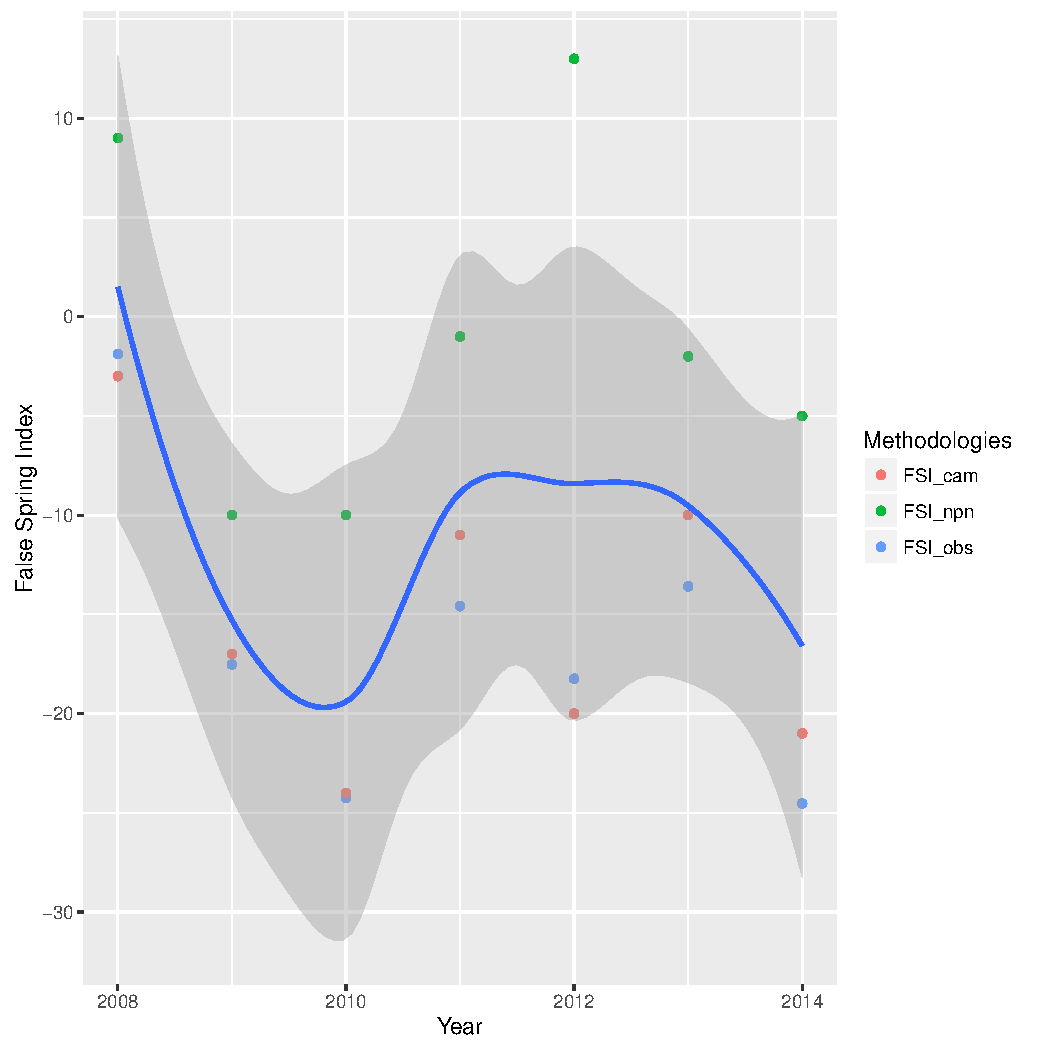
\includegraphics[width=\maxwidth]{figure/fsifig-1} \caption[A scatterplot indicating FSI values from 2008 to 2014 for each methdology used in this study]{A scatterplot indicating FSI values from 2008 to 2014 for each methdology used in this study. PhenoCam FSI values are red, Observed FSI values are blue, and USA-NPN FSI values are green.}\label{fig:fsifig}
\end{figure}




The false spring equation also requires a last freeze date input. There are two types of freezes: a ``hard freeze" at -2.2$^{\circ}$C and a ``soft freeze" at -1.7$^{\circ}$C \citep{Vavrus2006, Kodra2011, Augspurger2013}. However, these definitions are still largely under debate. There are numerous definitions of freezes and various requirements for damaging spring temperatures (Table \ref{tab:temperature}), making it extremely difficult to determine when the last freeze date is in the spring. Future false spring equations must integrate species, life stage, and habitat differences in temperature thresholds in order to accurately determine level of damage sustained by a false spring event.
 
\begin{landscape}
\begin{center}
\captionof{table}{Comparing damaging spring temperature thresholds in ecological and agronomical studies across various species and phenophases.} \label{tab:temperature} 
\footnotesize
\begin{tabular}{|c | c | c | c | c | c|}
\hline
\textbf{Sector} & \textbf{BBCH} & \textbf{Species} & \textbf{Temperature ($^{\circ}$C)} & \textbf{Type} & \textbf{Source} \\
\hline
Ecological & 9-15 & Sorbus aucuparia & -7.4 & 50\% lethality & \cite{Lenz2016} \\
\hline
Ecological & 9-15 & Prunus avium & -8.5 & 50\% lethality & \cite{Lenz2016} \\
\hline
Ecological & 9-15 & Tilia platyphyllos & -7.4 & 50\% lethality & \cite{Lenz2016} \\
\hline
Ecological & 9-15 & Acer pseudoplatanus & -6.7 & 50\% lethality & \cite{Lenz2016}\\
\hline
Ecological & 9-15 & Fagus sylvatica & -4.8 & 50\% lethality & \cite{Lenz2016}\\
\hline
Ecological & 9+ & All & -2.2 & hard & \cite{Schwartz1993}\\
\hline
Ecological & 9+ & All & -1.7 & soft & \cite{Augspurger2013} \\
\hline
Ecological & All & All & 2 SD below winter TAVG & cold-air outbreaks & \cite{Vavrus2006} \\
\hline
Ecological & 9+ & Eucalyptus pauciflora & -5.8 & elevated CO2 and temperature threshold & \cite{Barker2005} \\
\hline
Ecological & 9+ & All & -2.2 & 7 day threshold & \cite{Peterson2014} \\
\hline
Agrinomical & 9+ & All & 2 & Risk threshold for clear nights & \cite{Cannell1986} \\
\hline
Agrinomical & Floral & Vaccinium spp. & -4.4 to 0 & sprinkler protection threshold & \cite{Longstroth2012} \\
\hline
Agrinomical & 9 & Rosaceae & -7.2 & 10\% lethality & \cite{Longstroth2013}\\
\hline
Agrinomical & 9 & Rosaceae & -13.3 & 90\% lethality & \cite{Longstroth2013} \\
\hline
Agrinomical & All & All & Varies & Radiation Frost & \cite{Barlow2015} \\
\hline
Agrinomical & Floral & Wheat & -4 to -5 & 10-90\% lethality & \cite{Barlow2015} \\
\hline
Agrinomical & Vegetative & Wheat & -7 for 2hrs & 100\% lethality & \cite{Barlow2015} \\
\hline
Agrinomical & Vegetative & Rice & 4.7 & lethal limit & \cite{Sanchez2013} \\
\hline
Agrinomical & Vegetative & Corn & -1.8 & lethal limit & \cite{Sanchez2013}\\
\hline
Agrinomical & Vegetative & Wheat & -17.2 & lethal limit & \cite{Sanchez2013} \\
\hline
\end{tabular}
\end{center}
\end{landscape}
\restoregeometry


\section*{Defining Vegetative Risk}
Different species respond differently to anthropogenic climate change. Most species are expected to begin leafout earlier in the season with warming spring temperatures but some species may have the opposite response \citep{Cleland2006, Yu2010, Xin2016}. Studies indicate that species growing at more northern latitudes tend to respond greater to photoperiod than species growing further south \citep {Partanen2004, Viheraaarnio2006, Caffarra2011}. Similarly, late successional species exhibit greater photoperiod sensitivities than pioneer or understory species \citep{Basler2012} and they also require more chilling in the winter and greater forcing temperatures in the spring to initiate budburst \citep{Laube2013}. It is anticipated that these more opportunistic individuals that initiate budburst earlier in the spring would attempt to limit freezing risk by increasing the rate of budburst and progress to full leaf expansion faster.

Reproductive phases are generally more sensitive to false spring events than vegetative phases. \citep{Augspurger2009, Lenz2013}. However, false spring events that occur during the vegetative growth phenophases impose the greatest freezing threat to deciduous tree and shrub species because plants will suffer greater long-term effects from the loss of photosynthetic tissue than trees that lose one year of reproductive growth \citep{Sakai1987}. Plants at certain vegetative phenophases (i.e. before full leafout of the entire plant) are more likely to sustain damage from a false spring than individuals past the leafout phenophase. Therefore, spring phenology is a crucial indicator for how much damage a plant will sustain from a freezing event.

The rate of budburst and the length of time between budburst and leafout is essential for predicting level of damage from a false spring event. We will refer to the timing of these collective phenophases (i.e. budburst to leafout) as the duration of vegetative risk. The duration of vegetative risk is usually extended if a freezing event occurs during the phenophases between budburst and full leafout. Species with short durations of vegetative risk often sustain higher levels of damage \citep {Augspurger2009}. It is hypothesized that if the duration of vegetative risk is longer, then the buds and leaves will be heartier against frosts, however this has yet to be tested thoroughly. We assess the interaction between duration of vegetative risk and false spring events using two datasets: from a growth chamber chilling experiment and long-term observational data.

\subsection*{Dan's Data} % Need title
Deciduous trees and shrubs require a certain number of chilling hours in order to leave the endodormancy phase. This helps protect temperate plants against stochastic warm spells in the winter so that they do not break dormancy too early in the season. Chilling units differ across species and across habitats. Species growing at higher latitudes are more likely to have lower chilling requirements to break dormancy \citep{Myking1995, Howe2003} in order to optimize growing season length \citep{Prevey2017}. % Lizzie, should I avoid this Prevey reference? 
With anthropogenic climate change, it is possible that certain species will have insufficient winter chilling (especially at lower latitudes) resulting in higher spring forcing requirements \citep{McCreary1990, Morin2009, Fu2012, Polgar2014, Chuine2010}. Similarly, spring forcing temperature and photoperiod cues for budburst to occur vary among species and habitats, which is evident through the high levels of genetic diversity across temperate forest tree species \citep{Chuine2001}. Data from a growth chamber experiment were used to compare 9 temperate forest species between two treatments: high chilling hours, long photoperiod and high forcing temperatures (WL1) against no additional chilling, short photoperiod and low forcing temperatures (CS0) (Flynn and Wolkovich, 2017?).

According to the results, individuals that initiate budburst earlier in the season (i.e. {\textit {Betula papyrifera}} (Marsh.) and {\textit{Ilex mucronata}} (L.)) tend to initiate budburst early regardless of treatment, but the treatment does affect the duration of vegetative risk significantly (Figure \ref{fig:dan}). As the season progresses, treatment does not affect the duration of vegetative risk as much, however, the day of budburst tends to be later in the season with the weaker treatment effects (i.e. CS0). Anova results indicate forcing temperatures and photoperiod length determine the duration of vegetative risk more than chilling requirements. This could indicate that chilling influences budburst and leafout similarly, while photoperiod and forcing temperatures have varying effects on the two phenophases. Further studies are essential to investigate the interplay between chilling, forcing, and photoperiod effects on the duration of vegetative risk, especially for species occupying habitats more susceptible to false spring events.

\begin{figure}[H]
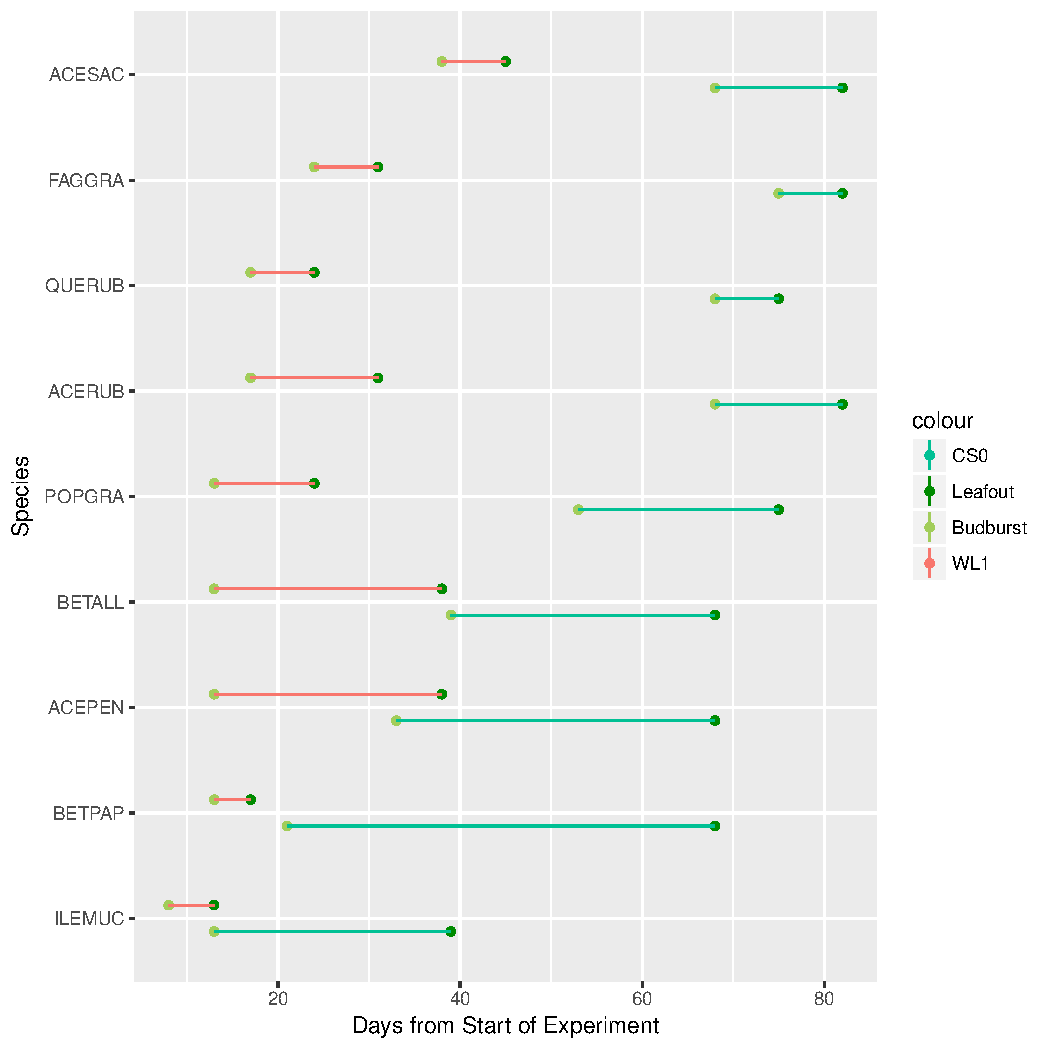
\includegraphics[width=\maxwidth]{figure/dan-1} \caption[Day of budburst and the day of leaf out for native tree species in New England]{Day of budburst and the day of leaf out for native tree species in New England. Data was collected from a growth chamber experiment using any combination of two photoperiod treatments, two forcing treatments, and three chilling treatments. The standard deviation is represented in blue for budburst and green for leaf out.}\label{fig:dan}
\end{figure}




\subsection*{Observational Data} %Needs new title!
Forcing temperatures in the spring affect the duration of vegetative risk: years with lower forcing temperatures and fewer growing degree days will have longer durations of vegetative risk \citep{Donnelly2017}. It is therefore expected that high variation in spring temperatures (i.e. oscillating above and below the development threshold) may result in longer durations of vegetative risk. Using observational data from Harvard Forest \citep{Okeefe2014}, we compared two years of data: one year that had an unusually early spring onset (2010) and another year that an unusually late spring onset (2014). By comparing the durations of vegetative risk to the growing degree days for each year, we found that the number of growing degree days were highly comparable for both years, however, in 2010, the duration of vegetative risk was slightly longer overall (Figure \ref{fig:forest}). This could potentially be due to photoperiodic effects. Forcing temperature requirements, like chilling requirements, are key phenotypic traits for many temperate tree species \citep{Kramer2017}, which may explain the similarity in the relationship between growing degree days and budburst date across the two years.

\begin{figure} [H] 
\begin{center}
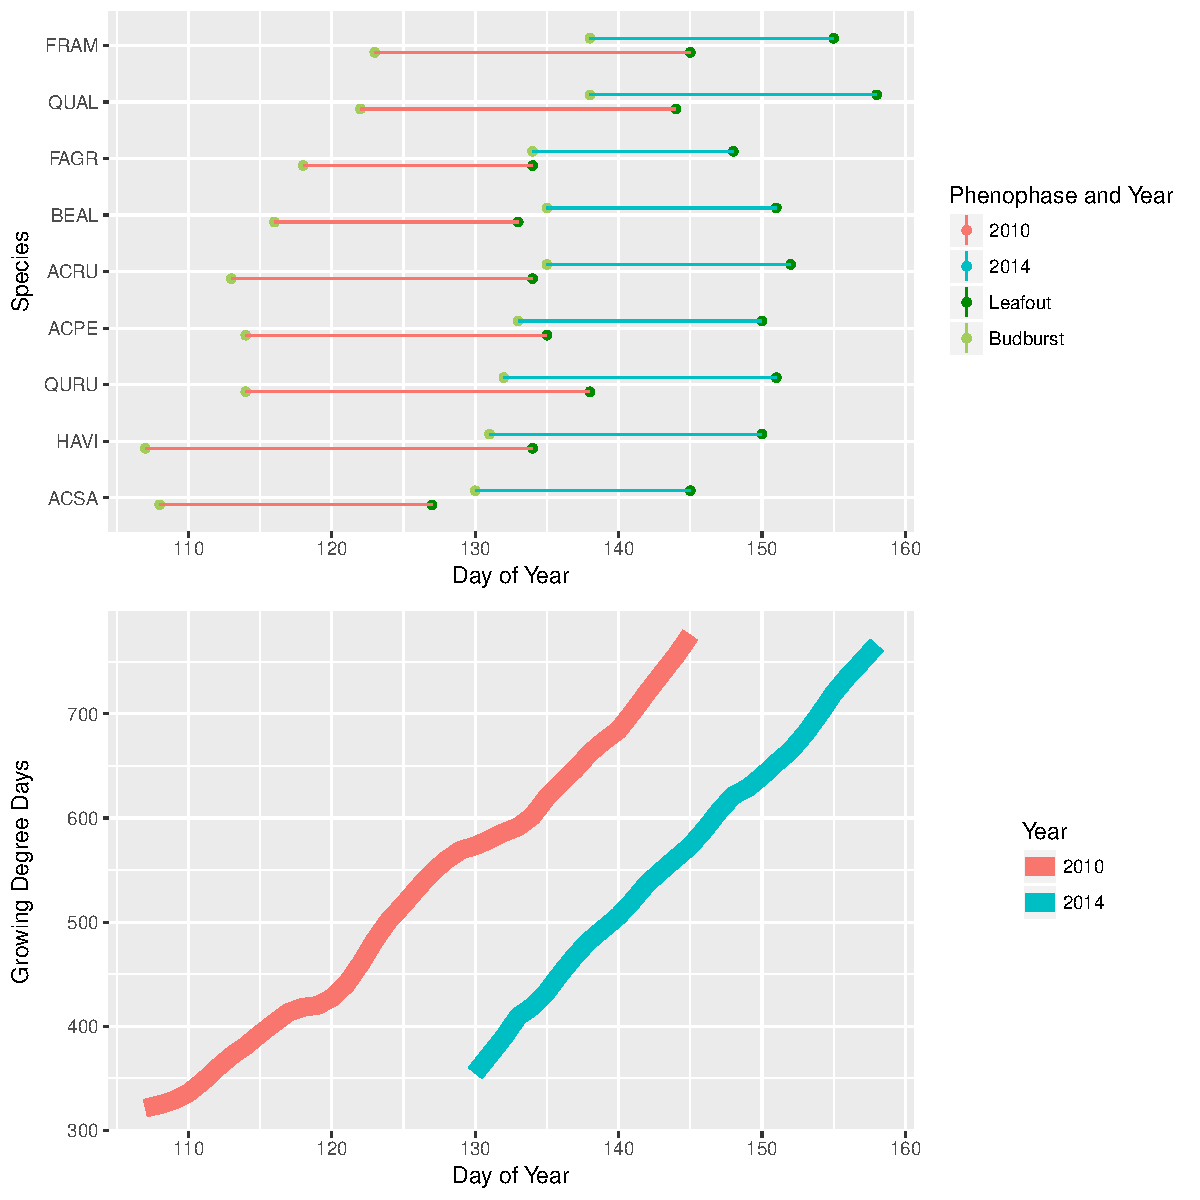
\includegraphics{..//figure/HF_gddTime.pdf}
\caption{A comparison of two years of observational data investigating the effects of growing degree days on the duration of vegetative risk. The average duration of vegetative risk for 2010 was 21 +/- 3.39 days versus 17.1 +/- 1.96 days in 2014.}\label{fig:forest}
\end{center}
\end{figure}

\section*{Regional Differences in False Spring Risk and Temperature Thresholds}
Climatic variation across regions results in varying durations of vegetative risk due to different photoperiod lengths and forcing temperatures. Species distributions are largely driven by phenology \citep{Chuine2001} and photoinsensitive species are likely to out compete photosensitive species as spring forcing temperatures continue to increase \citep{Vitasse2011,Gauzere2017}. However, the climatic implications of increasing forcing temperatures could potentially lead to earlier dates of budburst and enhance the risk for frost or drought risk. These shifts in climatic regimes could vary in intensity across regions (i.e. habitats currently at risk of false spring damage could become low risk regions over time). There are discrepancies in defining a false spring event, especially with understanding damaging freezing temperatures. Some regions and species may be more able to tolerate lower temperature thresholds than others (Table \ref{tab:temperature}). It is crucial to gain an understanding on which climatic parameters result in false spring events and also to understand what habitats are at risk now and what habitats will be at risk in the future. It is anticipated that most habitats will trend towards earlier spring onsets, however, last freeze dates will not occur at the same rate, rendering some regions to be more susceptible to false spring events in the future \citep{Labe2016}. 

By determining the average time of budburst to leafout dates for the dominant species in five archetypal climate regions, we were able to estimate the current spatial variation of false spring risk (Figure \ref{fig:regional}). We assessed the number of freeze days (-2.2$^{\circ}$C) \citep{Schwartz1993} that occurred on average over the past 50 years within the date ranges for each region. We found that Maine has the highest risk for frost damage and Lyon, France as the lowest (Figure \ref{fig:regional}). Current studies focus on latitudinal and photoperiodic effects \citep{Partanen2004, Viheraaarnio2006, Caffarra2011, Gauzere2017}, however, future research should aim to integrate spatiotemporal effects more when investigating false spring risk.

\begin{figure} [H] 
\begin{center}
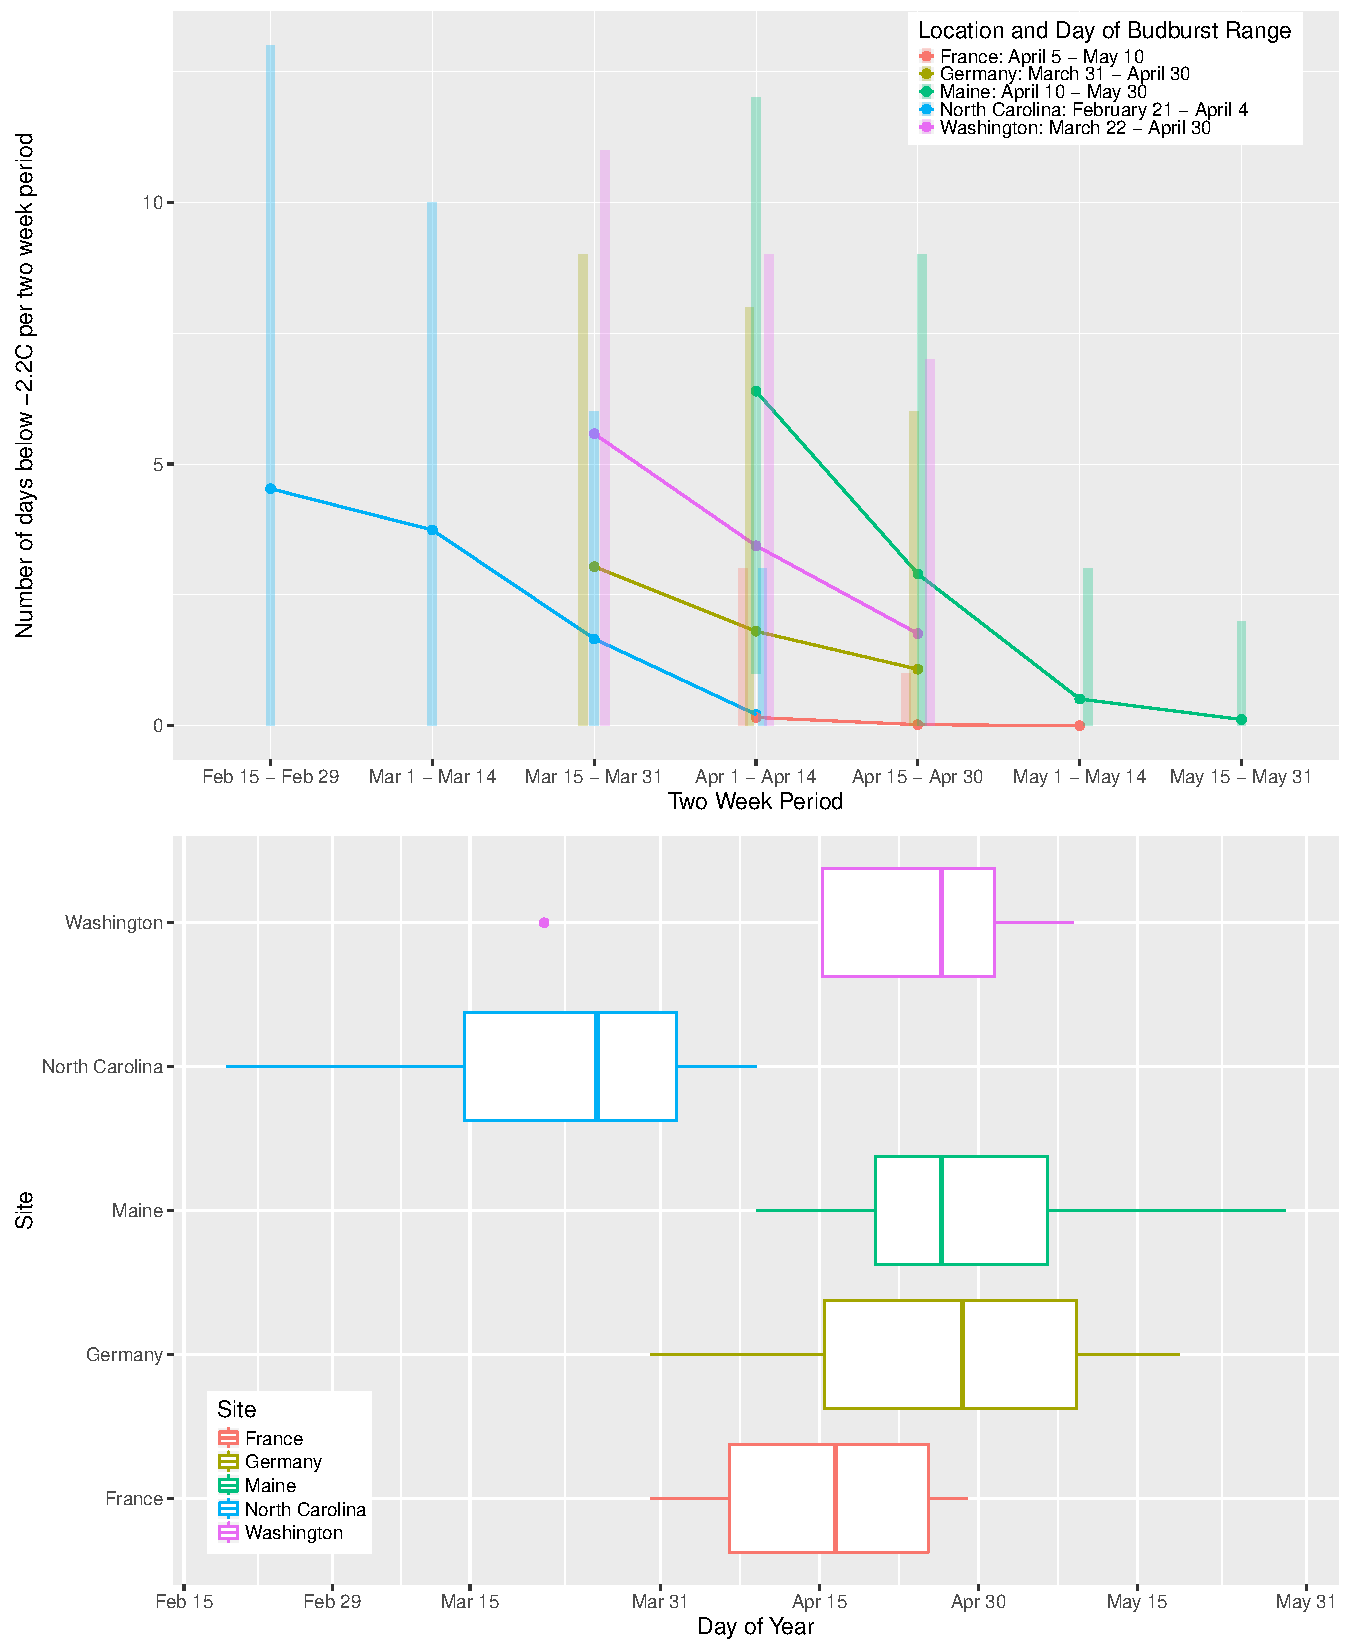
\includegraphics[width=16cm, height=13cm]{..//figure/RegionalRisk.pdf} 
\caption{A comparison of false spring risk across five climate regions. The data was subsetted for each region based on earliest historical spring onset date to the latest historical leafout date and was divided into biweekly time periods \citep{Schaber2005, White2009, Soudani2012, USA-NPN2016}.}\label{fig:regional} 
\end{center}
\end{figure}

\section*{Conclusion}
As global change progresses and atmospheric CO$_{\text{2}}$ increases, false spring damage will likely worsen and low temperature thresholds will decrease (Table \ref{tab:temperature}) \citep{Beerling2001, Barker2005}. Plants have higher freeze tolerance after exposure to low temperatures over a period of time \citep{Thomashow1999} so shorter dormancy lengths coupled with elevated CO$_{\text{2}}$ levels could result in highly detrimental effects from false spring events. Ecosystem dynamics and risk of damage can vary from year to year and the timing between last freeze date and date of spring onset may become less consistent. With warm temperatures advancing in the spring but last spring freeze dates staying the same, there could potentially be more damaging events in the future, especially in high risk regions \citep{Gu2008, Inouye2008}. This shift in timing could result in more events where understory species leaf out prior to the last freeze and escape frost damage but canopy species may be at higher risk, thus potentially resulting in crown dieback for the larger tree species and subsequently enhanced sun exposure and damage to understory species. False spring events could also adversely affect other trophic levels if fruit and seed development is impacted \citep{Gu2008}, making false spring studies even more ecologically significant.

Phenology is closely linked to climatic regimes \citep{Wolkovich2011} and is therefore a key indicator in phenotypic variation for cold adpated traits and false spring risk avoidance. Understanding the variation of spring onset across regions and within habitats as well as the rate of budburst will permit greater insight into false spring risk. Tree species with smaller and more fragmented distribution ranges are more at risk to stochastic events (i.e. frost and drought) \citep{Alberto2013}. Therefore, it is essential that temperate forest tree species maintain continuous ranges in order to successfully track the changes in climate and to utilize photoperiodic and temperature cues simultaneously rather than rely strictly on photoperiodism - especially along range edges \citep{Zohner2016, Gauzere2017}. Future studies are necessary to investigate the relationship between anthropogenic climate change, spatiotemporal factors, the duration of vegetative risk, and the level of damage sustained from false spring events

By utilizing only two simple metrics (last freeze date and spring onset date), researchers fail to assess the myriad of factors essential in determining false spring risk and damage. Future studies are necessary to gain an understanding with relationships between species, functional group, phenophase, and region and the differences in false spring damage. It is also essential that a temperature threshold is established for all functional types and phenophases across regions in order to effectively predict false spring risk in the future. An integrated approach to assessing past and future spring freeze damage must be realized as global climate change progresses in order to mitigate the adverse ecological and economic effects of false springs.

\bibliography{..//refs/SpringFreeze.bib}

\section*{Supplemental Information}
% latex table generated in R 3.2.2 by xtable 1.8-2 package
% Sat Jul  1 12:13:24 2017
\begin{table}[ht]
\centering
\begin{tabular}{rrrrr}
  \hline
  ACEPEN & Sum.Sq & Df & F value & Pr(>F) \\
 \hline
chilling & 149.41 &   2 & 1.20 & 0.30 \\ 
  forcing & 4909.59 &   1 & 78.94 & 0.00 \\ 
  photoperiod & 1309.59 &   1 & 21.06 & 0.00 \\ 
  Residuals & 6654.56 & 107 &  &  \\ 
   \hline
\end{tabular}
\end{table}
% latex table generated in R 3.2.2 by xtable 1.8-2 package
% Sat Jul  1 12:13:24 2017
\begin{table}[ht]
\centering
\begin{tabular}{rrrrr}
  \hline
  ACERUB & Sum.Sq & Df & F value & Pr(>F) \\
 \hline
chilling & 0.62 &   2 & 0.00 & 1.00 \\ 
  forcing & 1731.00 &   1 & 25.92 & 0.00 \\ 
  photoperiod & 462.78 &   1 & 6.93 & 0.01 \\ 
  Residuals & 6611.17 &  99 &  &  \\ 
   \hline
\end{tabular}
\end{table}
% latex table generated in R 3.2.2 by xtable 1.8-2 package
% Sat Jul  1 12:13:24 2017
\begin{table}[ht]
\centering
\begin{tabular}{rrrrr}
  \hline
  ACESAC & Sum.Sq & Df & F value & Pr(>F) \\
 \hline
chilling & 65.41 &   2 & 0.46 & 0.64 \\ 
  forcing & 259.14 &   1 & 3.61 & 0.06 \\ 
  photoperiod & 231.41 &   1 & 3.22 & 0.08 \\ 
  Residuals & 4524.88 &  63 &  &  \\ 
   \hline
\end{tabular}
\end{table}
% latex table generated in R 3.2.2 by xtable 1.8-2 package
% Sat Jul  1 12:13:24 2017
\begin{table}[ht]
\centering
\begin{tabular}{rrrrr}
  \hline
  BETALL & Sum.Sq & Df & F value & Pr(>F) \\
 \hline
chilling & 525.95 &   2 & 5.00 & 0.01 \\ 
  forcing & 1463.30 &   1 & 27.81 & 0.00 \\ 
  photoperiod & 632.83 &   1 & 12.03 & 0.00 \\ 
  Residuals & 6944.50 & 132 &  &  \\ 
   \hline
\end{tabular}
\end{table}
% latex table generated in R 3.2.2 by xtable 1.8-2 package
% Sat Jul  1 12:13:24 2017
\begin{table}[ht]
\centering
\begin{tabular}{rrrrr}
  \hline
  BETPAP & Sum.Sq & Df & F value & Pr(>F) \\
 \hline
chilling & 6.00 &   2 & 0.04 & 0.96 \\ 
  forcing & 1776.23 &   1 & 21.47 & 0.00 \\ 
  photoperiod & 1105.08 &   1 & 13.35 & 0.00 \\ 
  Residuals & 10509.00 & 127 &  &  \\ 
   \hline
\end{tabular}
\end{table}
% latex table generated in R 3.2.2 by xtable 1.8-2 package
% Sat Jul  1 12:13:24 2017
\begin{table}[ht]
\centering
\begin{tabular}{rrrrr}
  \hline
  FAGGRA & Sum.Sq & Df & F value & Pr(>F) \\
 \hline
chilling & 144.41 &   2 & 1.66 & 0.20 \\ 
  forcing & 611.20 &   1 & 14.04 & 0.00 \\ 
  photoperiod & 1.05 &   1 & 0.02 & 0.88 \\ 
  Residuals & 2829.78 &  65 &  &  \\ 
   \hline
\end{tabular}
\end{table}
% latex table generated in R 3.2.2 by xtable 1.8-2 package
% Sat Jul  1 12:13:24 2017
\begin{table}[ht]
\centering
\begin{tabular}{rrrrr}
  \hline
  ILEMUC & Sum.Sq & Df & F value & Pr(>F) \\
 \hline
chilling & 26.49 &   2 & 0.54 & 0.59 \\ 
  forcing & 2262.34 &   1 & 91.61 & 0.00 \\ 
  photoperiod & 1035.85 &   1 & 41.94 & 0.00 \\ 
  Residuals & 3334.05 & 135 &  &  \\ 
   \hline
\end{tabular}
\end{table}
% latex table generated in R 3.2.2 by xtable 1.8-2 package
% Sat Jul  1 12:13:24 2017
\begin{table}[ht]
\centering
\begin{tabular}{rrrrr}
  \hline
  POPGRA & Sum.Sq & Df & F value & Pr(>F) \\
 \hline
chilling & 54.63 &   2 & 0.39 & 0.68 \\ 
  forcing & 2405.73 &   1 & 34.52 & 0.00 \\ 
  photoperiod & 1019.78 &   1 & 14.63 & 0.00 \\ 
  Residuals & 6760.98 &  97 &  &  \\ 
   \hline
\end{tabular}
\end{table}
% latex table generated in R 3.2.2 by xtable 1.8-2 package
% Sat Jul  1 12:13:24 2017
\begin{table}[ht]
\centering
\begin{tabular}{rrrrr}
  \hline
  QUERUB & Sum.Sq & Df & F value & Pr(>F) \\
 \hline
chilling & 35.61 &   2 & 0.45 & 0.64 \\ 
  forcing & 680.83 &   1 & 17.34 & 0.00 \\ 
  photoperiod & 369.53 &   1 & 9.41 & 0.00 \\ 
  Residuals & 4946.29 & 126 &  &  \\ 
   \hline
\end{tabular}
\end{table}


% latex table generated in R 3.2.2 by xtable 1.8-2 package
% Sat Jul  1 12:13:24 2017
\begin{table}[ht]
\centering
\begin{tabular}{rrrrr}
  \hline
  ACEPEN & Sum.Sq & Df & F value & Pr(>F) \\
 \hline
chilling & 104.66 &   2 & 0.87 & 0.42 \\ 
  forcing & 4745.38 &   1 & 79.18 & 0.00 \\ 
  photoperiod & 1306.03 &   1 & 21.79 & 0.00 \\ 
  chilling:forcing & 63.31 &   2 & 0.53 & 0.59 \\ 
  chilling:photoperiod & 181.96 &   2 & 1.52 & 0.22 \\ 
  forcing:photoperiod & 257.63 &   1 & 4.30 & 0.04 \\ 
  Residuals & 6113.18 & 102 &  &  \\ 
   \hline
\end{tabular}
\end{table}
% latex table generated in R 3.2.2 by xtable 1.8-2 package
% Sat Jul  1 12:13:24 2017
\begin{table}[ht]
\centering
\begin{tabular}{rrrrr}
  \hline
  ACERUB & Sum.Sq & Df & F value & Pr(>F) \\
 \hline
chilling & 1.53 &   2 & 0.01 & 0.99 \\ 
  forcing & 1721.25 &   1 & 26.13 & 0.00 \\ 
  photoperiod & 381.81 &   1 & 5.80 & 0.02 \\ 
  chilling:forcing & 358.58 &   2 & 2.72 & 0.07 \\ 
  chilling:photoperiod & 37.69 &   2 & 0.29 & 0.75 \\ 
  forcing:photoperiod & 17.35 &   1 & 0.26 & 0.61 \\ 
  Residuals & 6191.98 &  94 &  &  \\ 
   \hline
\end{tabular}
\end{table}
% latex table generated in R 3.2.2 by xtable 1.8-2 package
% Sat Jul  1 12:13:24 2017
\begin{table}[ht]
\centering
\begin{tabular}{rrrrr}
  \hline
  ACESAC & Sum.Sq & Df & F value & Pr(>F) \\
 \hline
chilling & 65.78 &   2 & 0.45 & 0.64 \\ 
  forcing & 204.31 &   1 & 2.83 & 0.10 \\ 
  photoperiod & 267.24 &   1 & 3.70 & 0.06 \\ 
  chilling:forcing & 76.27 &   2 & 0.53 & 0.59 \\ 
  chilling:photoperiod & 164.28 &   2 & 1.14 & 0.33 \\ 
  forcing:photoperiod & 0.05 &   1 & 0.00 & 0.98 \\ 
  Residuals & 4194.28 &  58 &  &  \\ 
   \hline
\end{tabular}
\end{table}
% latex table generated in R 3.2.2 by xtable 1.8-2 package
% Sat Jul  1 12:13:24 2017
\begin{table}[ht]
\centering
\begin{tabular}{rrrrr}
  \hline
  BETALL & Sum.Sq & Df & F value & Pr(>F) \\
 \hline
chilling & 526.41 &   2 & 5.57 & 0.00 \\ 
  forcing & 1463.33 &   1 & 30.95 & 0.00 \\ 
  photoperiod & 632.83 &   1 & 13.38 & 0.00 \\ 
  chilling:forcing & 66.32 &   2 & 0.70 & 0.50 \\ 
  chilling:photoperiod & 226.18 &   2 & 2.39 & 0.10 \\ 
  forcing:photoperiod & 612.56 &   1 & 12.95 & 0.00 \\ 
  Residuals & 6005.50 & 127 &  &  \\ 
   \hline
\end{tabular}
\end{table}
% latex table generated in R 3.2.2 by xtable 1.8-2 package
% Sat Jul  1 12:13:24 2017
\begin{table}[ht]
\centering
\begin{tabular}{rrrrr}
  \hline
  BETPAP & Sum.Sq & Df & F value & Pr(>F) \\
 \hline
chilling & 6.07 &   2 & 0.04 & 0.96 \\ 
  forcing & 1765.57 &   1 & 21.22 & 0.00 \\ 
  photoperiod & 1101.18 &   1 & 13.24 & 0.00 \\ 
  chilling:forcing & 71.38 &   2 & 0.43 & 0.65 \\ 
  chilling:photoperiod & 62.92 &   2 & 0.38 & 0.69 \\ 
  forcing:photoperiod & 233.62 &   1 & 2.81 & 0.10 \\ 
  Residuals & 10148.80 & 122 &  &  \\ 
   \hline
\end{tabular}
\end{table}
% latex table generated in R 3.2.2 by xtable 1.8-2 package
% Sat Jul  1 12:13:24 2017
\begin{table}[ht]
\centering
\begin{tabular}{rrrrr}
  \hline
  FAGGRA & Sum.Sq & Df & F value & Pr(>F) \\
 \hline
chilling & 145.37 &   2 & 1.64 & 0.20 \\ 
  forcing & 595.26 &   1 & 13.40 & 0.00 \\ 
  photoperiod & 0.42 &   1 & 0.01 & 0.92 \\ 
  chilling:forcing & 39.45 &   2 & 0.44 & 0.64 \\ 
  chilling:photoperiod & 83.56 &   2 & 0.94 & 0.40 \\ 
  forcing:photoperiod & 35.33 &   1 & 0.80 & 0.38 \\ 
  Residuals & 2665.38 &  60 &  &  \\ 
   \hline
\end{tabular}
\end{table}
% latex table generated in R 3.2.2 by xtable 1.8-2 package
% Sat Jul  1 12:13:24 2017
\begin{table}[ht]
\centering
\begin{tabular}{rrrrr}
  \hline
  ILEMUC & Sum.Sq & Df & F value & Pr(>F) \\
 \hline
chilling & 28.03 &   2 & 0.60 & 0.55 \\ 
  forcing & 2277.73 &   1 & 97.37 & 0.00 \\ 
  photoperiod & 1033.49 &   1 & 44.18 & 0.00 \\ 
  chilling:forcing & 16.09 &   2 & 0.34 & 0.71 \\ 
  chilling:photoperiod & 106.28 &   2 & 2.27 & 0.11 \\ 
  forcing:photoperiod & 171.89 &   1 & 7.35 & 0.01 \\ 
  Residuals & 3041.00 & 130 &  &  \\ 
   \hline
\end{tabular}
\end{table}
% latex table generated in R 3.2.2 by xtable 1.8-2 package
% Sat Jul  1 12:13:24 2017
\begin{table}[ht]
\centering
\begin{tabular}{rrrrr}
  \hline
  POPGRA & Sum.Sq & Df & F value & Pr(>F) \\
 \hline
chilling & 50.56 &   2 & 0.37 & 0.69 \\ 
  forcing & 2390.66 &   1 & 35.16 & 0.00 \\ 
  photoperiod & 1016.39 &   1 & 14.95 & 0.00 \\ 
  chilling:forcing & 45.72 &   2 & 0.34 & 0.72 \\ 
  chilling:photoperiod & 152.02 &   2 & 1.12 & 0.33 \\ 
  forcing:photoperiod & 296.37 &   1 & 4.36 & 0.04 \\ 
  Residuals & 6254.69 &  92 &  &  \\ 
   \hline
\end{tabular}
\end{table}
% latex table generated in R 3.2.2 by xtable 1.8-2 package
% Sat Jul  1 12:13:24 2017
\begin{table}[ht]
\centering
\begin{tabular}{rrrrr}
  \hline
  QUERUB & Sum.Sq & Df & F value & Pr(>F) \\
 \hline
chilling & 35.70 &   2 & 0.46 & 0.63 \\ 
  forcing & 668.59 &   1 & 17.39 & 0.00 \\ 
  photoperiod & 364.39 &   1 & 9.48 & 0.00 \\ 
  chilling:forcing & 174.11 &   2 & 2.26 & 0.11 \\ 
  chilling:photoperiod & 110.91 &   2 & 1.44 & 0.24 \\ 
  forcing:photoperiod & 15.92 &   1 & 0.41 & 0.52 \\ 
  Residuals & 4652.62 & 121 &  &  \\ 
   \hline
\end{tabular}
\end{table}





\end{document}
